\documentclass[letterpaper,11pt]{article}
\oddsidemargin -1.0cm \textwidth 17.5cm

\usepackage[utf8]{inputenc}
\usepackage[activeacute,spanish, es-lcroman]{babel}
\decimalpoint
\usepackage{amsfonts,setspace}
\usepackage{amsmath}
\usepackage{amssymb, amsmath, amsthm}
\usepackage{comment}
\usepackage{float}
\usepackage{amssymb}
\usepackage{dsfont}
\usepackage{anysize}
\usepackage{multicol}
\usepackage{enumerate}
\usepackage{graphicx}
\usepackage[left=1.5cm,top=2cm,right=1.5cm, bottom=1.7cm]{geometry}
\setlength\headheight{1.5em} 
\usepackage{fancyhdr}
\usepackage{multicol}
\usepackage{hyperref}
\usepackage{wrapfig}
\usepackage{subcaption}
\usepackage{siunitx}
\usepackage{cancel}
\usepackage{mdwlist}
\usepackage{svg}
\pagestyle{fancy}
\fancyhf{}
\renewcommand{\labelenumi}{\normalsize\bfseries P\arabic{enumi}.}
\renewcommand{\labelenumii}{\normalsize\bfseries (\alph{enumii})}
\renewcommand{\labelenumiii}{\normalsize\bfseries \roman{enumiii})}


\begin{document}

\fancyhead[L]{\itshape{Facultad de Ciencias F\'isicas y Matem\'aticas}}
\fancyhead[R]{\itshape{Universidad de Chile}}

\begin{minipage}{11.5cm}
    \begin{flushleft}
        \hspace*{-0.6cm}\textbf{FI1000-1 Introducción a la Física Clásica}\\
        \hspace*{-0.6cm}\textbf{Profesora:} Jocelyn Dunstan\\
        \hspace*{-0.6cm}\textbf{Auxiliar:} Alejandro Silva\\
        \hspace*{-0.6cm}\textbf{Ayudantes:} Macarena Muñoz \& Catalina Vargas\\
    \end{flushleft}
\end{minipage}

\begin{picture}(2,3)
    \svgpath{../}  % descomentar si se agrega a carpeta "auxiliares"
    \put(366, 10){\includesvg[scale=0.31]{img/dfi.svg}}
\end{picture}

\begin{center}
	\LARGE\textbf{Auxiliar \#1}\\
	\Large{Trigonometría}
\end{center}

\vspace{-1.5cm}
\begin{enumerate}\setlength{\itemsep}{0.4cm}

\rfoot[]{pág. \thepage}

\item[]

\item Demuestre el teorema del seno y del coseno para un triángulo obtusángulo\\
\textbf{\textit{Hint:}} forme un triángulo rectángulo

\begin{figure}[H]
    \centering
    \begin{subfigure}[t]{0.6\textwidth}
        \centering
        \svgpath{../img/aux1}
        \includesvg[width=0.65\linewidth]{triangulo.svg}
    \end{subfigure}
    \hspace{1em}
    \begin{subfigure}[b]{0.30\textwidth}
        $\cdot$ Teo. seno:
        \begin{align*}
            \frac{\sin{\alpha}}{a}=\frac{\sin{\beta}}{b}=\frac{\sin{\gamma}}{c}
        \end{align*}
        
        $\cdot$ Teo. coseno:
        \begin{align*}
            a^2 &= b^2 + c^2 -2bc\cos{\alpha}\\
            b^2 &= a^2 + c^2 -2ac\cos{\beta}\\
            c^2 &= a^2 + b^2 -2ab\cos{\gamma}
        \end{align*}
    \end{subfigure}
\end{figure}

\item Una persona ubicada en el punto $P$ (ver Figura P2) observa dos montañas, una a la izquierda y otra a la derecha. Sean $\alpha$ y $\beta$ los ángulos de elevación de estas montañas. Si la montaña de la izquierda tiene una altura $h$ y la separación entre las proyecciones de las cimas sobre el nivel de la superficie terrestre es $D$, calcule la altura del otro monte. 


\begin{figure}[H]
    \centering
    \begin{subfigure}[t]{0.44\textwidth}
        \centering
        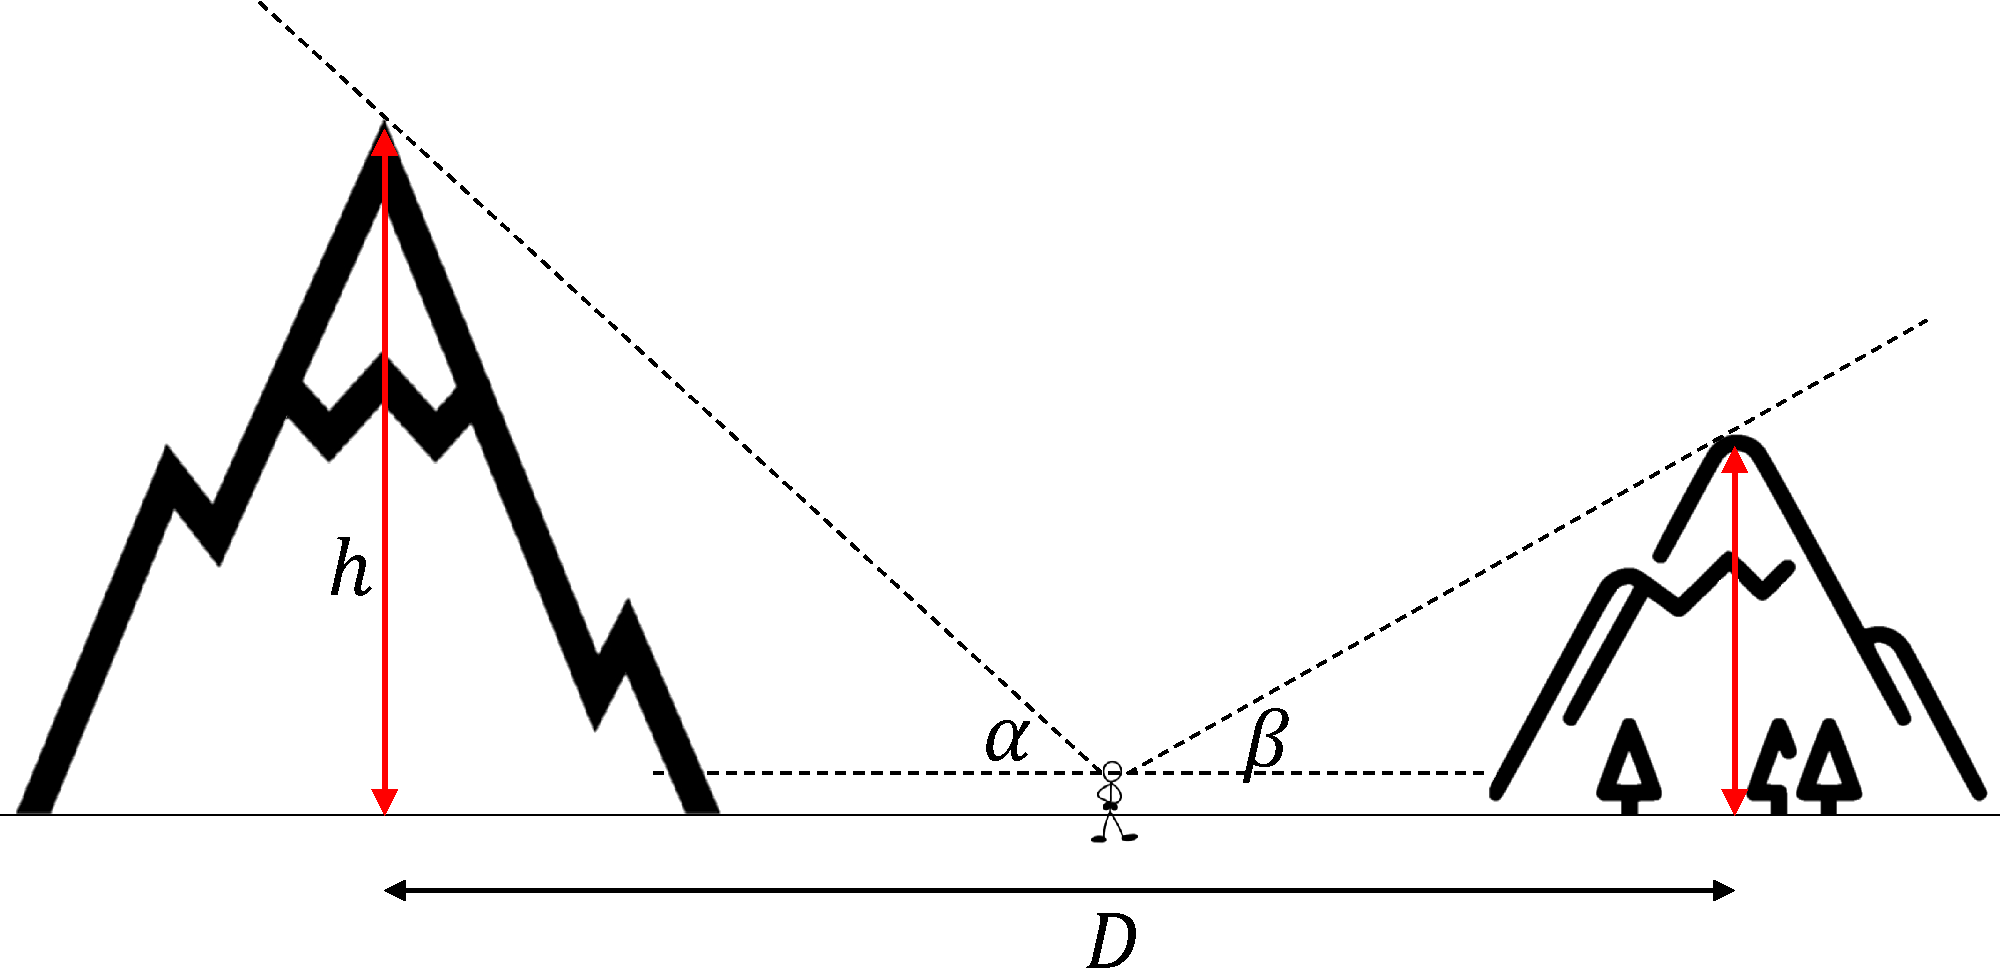
\includegraphics[width=0.95\linewidth]{2021-1/Imagenes/aux0/mountain.pdf}
        \caption{P2}
    \end{subfigure}
    \begin{subfigure}[t]{0.40\textwidth}
        \centering
        \svgpath{../img/aux1}
        \includesvg[width=0.82\linewidth]{tortugas.svg}
        \caption{P3}
    \end{subfigure}
\end{figure}

\item Una tortuga se encuentra al pie de un cerro cuya inclinación es $\gamma$. Desde cierta posición avista, con un ángulo de elevación $\alpha$ respecto al piso, a su compañera tortuga que se encuentra en la punta de un poste vertical ubicado en la cima del cerro. Luego, la tortuga avanza una distancia $d$ en dirección al poste. En este lugar avista a su compañera con un ángulo de elevación $\beta$. Encuentre la altura $h$ del poste en el que se encuentra la compañera tortuga. Analice el caso $\gamma\rightarrow 0$

\item \textbf{[Análisis Dimensional]} Realice un análisis dimensional a las siguientes expresiones de cinemática:
    
    {
    \begin{multicols}{3}
        \begin{enumerate}
        
        \item Ec. de itinerario:\\
        $y(t) = y_0 + v_0 t + \frac{1}{2} a t^2$
        
        \columnbreak
        
        \item Ec. de velocidad (?):\\
        $v(t) = v_0 + at$
        
        \columnbreak
        
        \item Ec. de Torricelli:\\
        $v_f^2 = v_i^2 + 2ad$
        
    \end{enumerate}
    \end{multicols}
    }

% Para imágenes vectoriales -> el texto tiene que estar en LaTeX
% \begin{figure}[htbp]
%   \centering
%   \svgpath{../Imagenes/ejercicios}  -> .. irse pa'trás 
%   \includesvg{ej5.svg}
% \end{figure}



\end{enumerate}
\end{document}
